% File: pram-example.tex
\documentclass{standalone}

\usepackage{tikz}
\usetikzlibrary{positioning, shapes, calc, backgrounds, fit}

\begin{document}
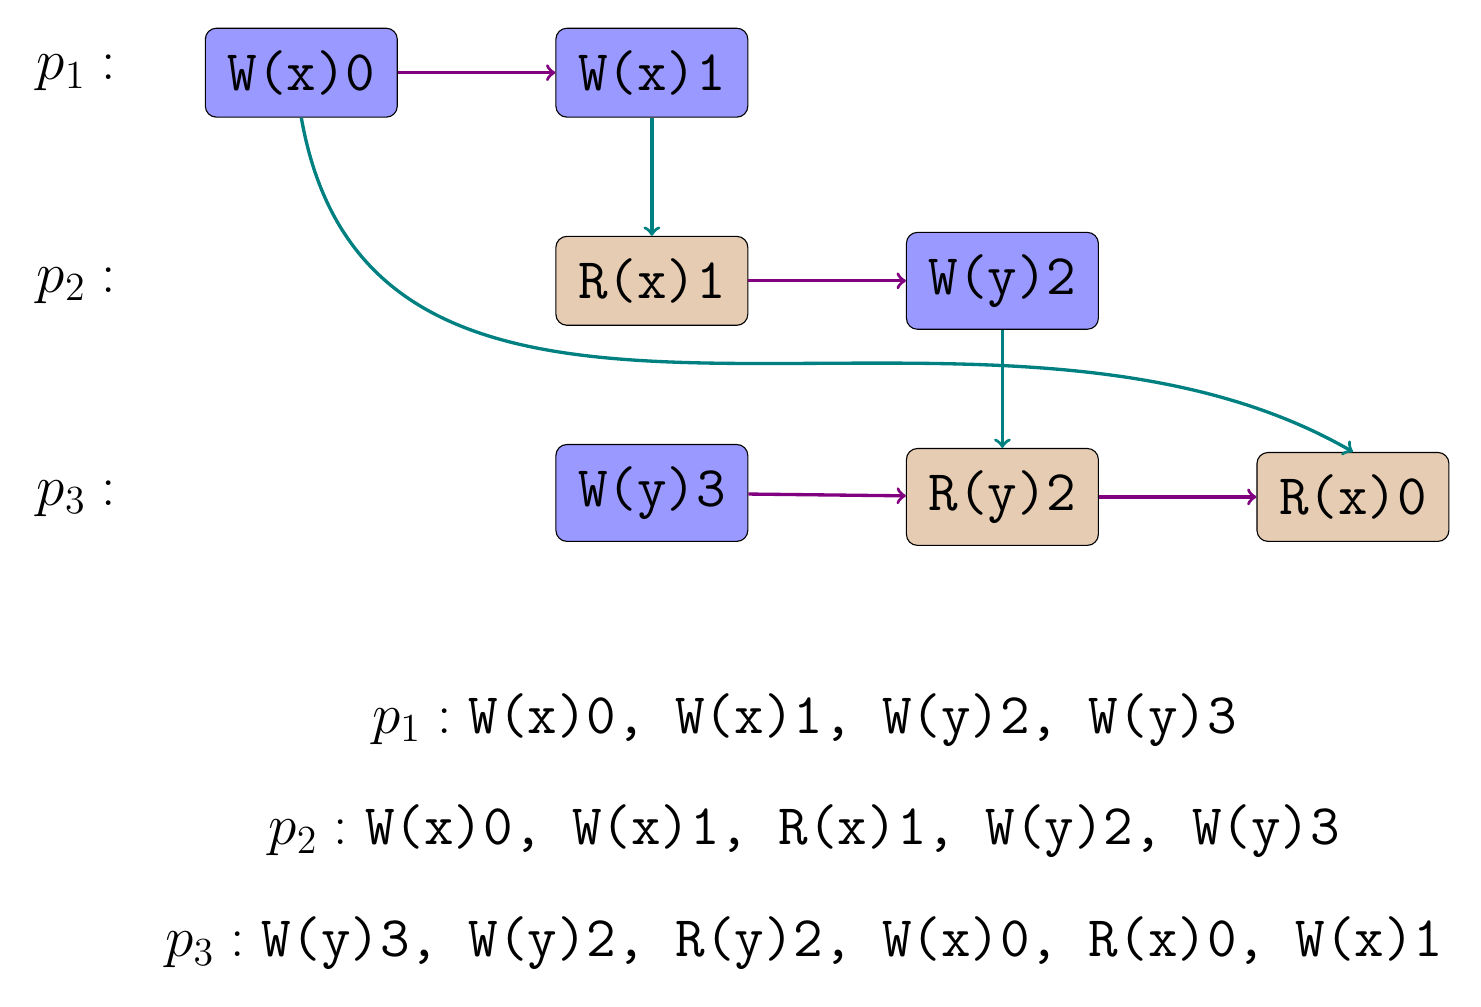
\begin{tikzpicture}[wop/.style = {rectangle, rounded corners, fill = blue!40, draw, font = \huge, 
  inner sep = 8pt}, rop/.style = {rectangle, rounded corners, fill = brown!40, draw, font = \huge, 
  inner sep = 8pt}, process/.style = {font = \huge}, po/.style = {->, very thick, violet}, 
rw/.style = {->, very thick, teal}]

  \node (p1) [process] {$p_1:$}; 
  \node (wx0) [wop, right = 1.0cm of p1] {\texttt{W(x)0}};
  \node (wx1) [wop, right = 2.0cm of wx0] {\texttt{W(x)1}};

  \node (p2) [process, below = 2.0cm of p1] {$p_2:$}; 
  \node (rx1) [rop, below = 1.5cm of wx1] {\texttt{R(x)1}};
  \node (wy2) [wop, right = 2.0cm of rx1] {\texttt{W(y)2}};

  \node (p3) [process, below = 2.0cm of p2] {$p_3:$}; 
  \node (wy3) [wop, below = 1.5cm of rx1] {\texttt{W(y)3}};
  \node (ry2) [rop, below = 1.5cm of wy2] {\texttt{R(y)2}};
  \node (rx0) [rop, right = 2.0cm of ry2] {\texttt{R(x)0}};
  
  \draw [po] (wx0) to (wx1);
  \draw [po] (rx1) to (wy2);
  \draw [po] (wy3) to (ry2);
  \draw [po] (ry2) to (rx0);

  \draw [rw] (wx0.south) to [out = -80, in = 150] (rx0.north);
  \draw [rw] (wx1) to (rx1);
  \draw [rw] (wy2) to (ry2);


  \node (p1-serial) [font = \huge, below right = 2.0cm and 3.0cm of p3] {$p_1:$ \texttt{W(x)0, W(x)1, W(y)2, W(y)3}}; 
  \node (p2-serial) [font = \huge, below = 0.5cm of p1-serial] {$p_2:$ \texttt{W(x)0, 
  W(x)1, R(x)1, W(y)2, W(y)3}};
  \node (p3-serial) [font = \huge, below = 0.5cm of p2-serial] {$p_3:$ \texttt{W(y)3, W(y)2, R(y)2, W(x)0, R(x)0, W(x)1}};

\end{tikzpicture}

\end{document}


